\chapter{Исследовательская часть}
В этом разделе будет продемонстрирована работа программы, а также
приведены результаты тестирования алгоритмов.

\section{Демонстрация работы программы}
На рисунке 4.1 приведена демонстрация работы программы.

\FloatBarrier
\begin{figure}[h]
	\begin{center}
		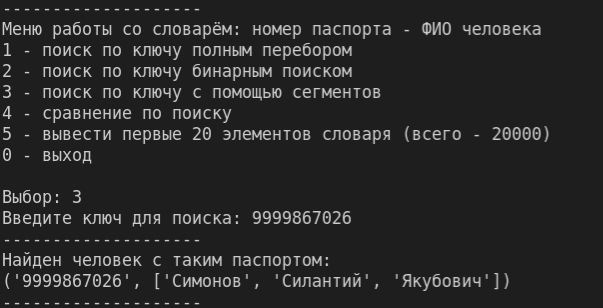
\includegraphics[]{inc/demostrate.png}
	\end{center}
	\caption{Демонстрация программы}
\end{figure}
\FloatBarrier


\section{Технические характеристики}
Технические характеристики устройства, на котором выполнялось тестирование, следующие:
\begin{itemize}
	\item операционная система: Ubuntu 20.04.1 LTS;
	\item память: 8 GB;
	\item процессор: Intel Core i5-1135G7 @ 2.40GHz \cite{intel}.
	\item количество ядер процессора: 8
\end{itemize}

Во время тестирования ноутбук был нагружен только встроенными приложениями окружения, а также непосредственно системой тестирования.

\section{Тестирование программы}
Тестирование будет производиться следующим образом.
Программа проводит поиск по каждому ключу всеми тремя алгоритмами 30 раз и усредняет полученные времена.
Затем строится график по каждому алгоритму.

Время измерялось в наносекундах. Во время не включалось создание сортированного массива для бинарного поиска и создание 
специального сегментированного словаря для третьего алгоритма.
На рисунке 4.2 представлены результаты тестирования алгоритмов.

\FloatBarrier
\begin{figure}[h]
	\begin{center}
		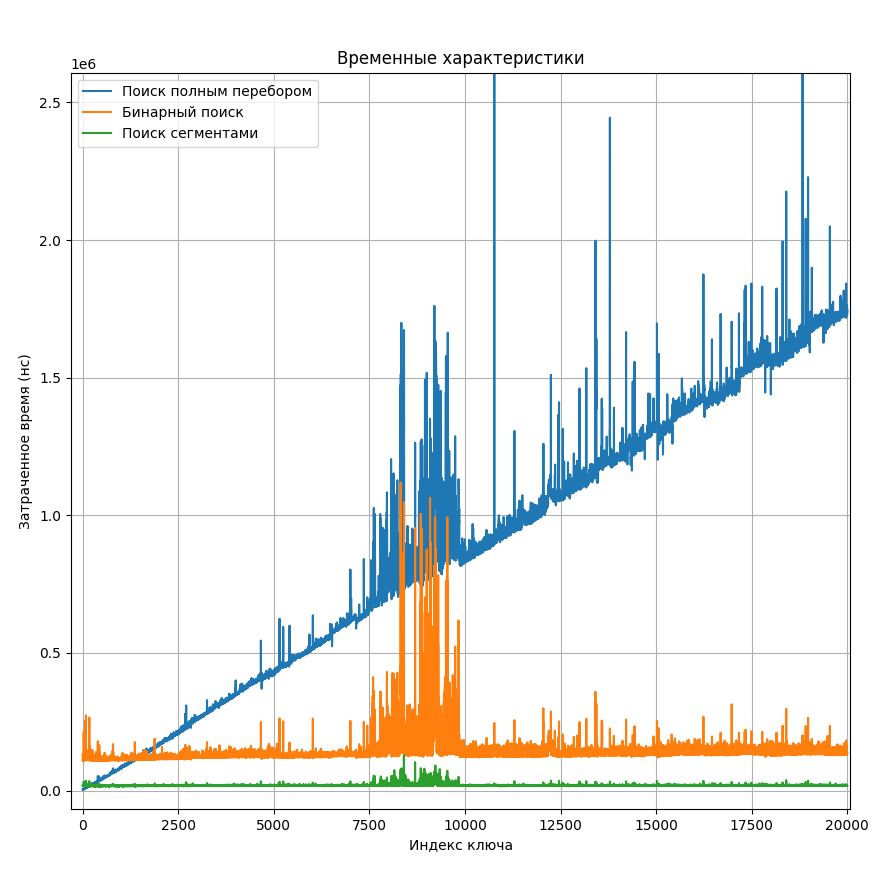
\includegraphics[width=\linewidth, height = 15cm]{inc/graph.png}
	\end{center}
	\caption{Демонстрация программы}
\end{figure}
\FloatBarrier

Перебор показал более стремительный рост по сравнению с остальными алгоритмами. 
На 20000-м ключе перебор оказался в семь раз медленнее, чем бинарный поиск, и в 70 раз медленнее, чем поиск с использованием сегментов.
На первой тысяче элементов бинарный поиск оказался самым медленным.
При этом время алгоритмов бинарного поиска и поиска с использованием сегментов практически не менялось в зависимости от номера ключа.

Также проведём тестирование алгоритмов по количеству операций сравнения в зависимости от ключа.
Результаты тестирования приведены в таблице 4.1

\FloatBarrier
\begin{table}[h]
	\caption{Результаты тестов}
	\centering
	\begin{tabular}{ | c | c | c | c |}
		\hline
		Ключ & Перебор & Бин.Поиск & Сегмент \\ 
		\hline
		6762048930 & 19984 & 15 & 11 \\
		0000023802 & 7405 & 14 & 20 \\
		9999867026 & 18700 & 15 & 17 \\
		9039639329 & 19964 & 12 & 16 \\
		8528870899 & 4003 & 15 & 13 \\
		8635632402 & 8058 & 14 & 13 \\
		1415792047 & 2048 & 15 & 10 \\
		7755312493 & 19981 & 13 & 16 \\
		0732110318 & 1 & 14 & 19 \\
		0506113949 & 19885 & 15 & 19 \\
		\hline
	\end{tabular}
\end{table}
\FloatBarrier

Видно, что для перебора количество сравнений зависит исключительно от того, каким по счёту ключ был добавлен в словарь.
Перебор оказался самым эффективным алгоритмом только для самых первых ключей в словаре.
У бинарного поиска и поиска с использованием сегментов количество сравнений не больше 20 для всех ключей.
Это не удивительно, так как последний алгоритм использует внутри себя тот же самый бинарный поиск.

Время у поиска с использованием сегментов на такое же количество операций уходит меньше времени, так как 
поиск проводится на существенно меньшем количестве элементов.

\section{Вывод}
Была продемонстрирована работа программы, и приведены результаты тестирования алгоритмов.
Поиск с использованием сегментов показал самое быстрое время практически на всех измерениях.
Обычный перебор ключей на 20000-м ключе оказался в семь раз медленнее, чем бинарный поиск, и в 70 раз медленнее, чем поиск с использованием сегментов.